\documentclass[main.tex]{subfiles}

\chapter{Contextualisation}

Dans ce chapitre, nous allons définir ce qu'est un Pokémon et ce qu'est les Video Game Championship (VGC).

\section{Caractéristiques}

Les Pokémon sont des créatures fictives vivant dans la franchise éponyme qui ont des caractéristiques de par leur apparence comme les couleurs, la forme et la taille mais on retrouve aussi des traits qui influe sur leurs prises d'actions durant certains évènements tels qu'en combat ou en concours comme nous l'avons défini précédemment. Le Pokémon peut progresser au travers de l'expérience et évoluer dans un nouveau Pokémon. Dans les parties suivantes nous allons définir ce qui compose un Pokémon et ce qui peut influer ces caractéristiques.

\subsection{Propre au Pokémon}

\subsubsection{Le niveau du Pokémon}

Un Pokémon peut aller du niveau 1 au niveau 100. Le niveau agit sur les statistiques du Pokémon, les augmentant au fur et à mesure qu'il progresse dans son niveau. Le niveau agit aussi sur les capacités qui peuvent ne peuvent appris qu'à un certain niveau ou après.

\subsubsection{Le sexe du Pokémon}

Un Pokémon peut être male, femelle ou asexué. Le sexe peut influer sur l'évolution du Pokémon changer le Pokémon qu'il peut devenir. Certains statuts, effets ou capacités peut aussi influer le Pokémon selon son sexe.

\subsubsection{Le type du Pokémon}
\label{type_pokemon}

Dans le monde Pokémon, les Pokémon peuvent avoir des types qu'ils leur sont attribués. Un pokémon a toujours un type qui lui est associé. Depuis la seconde génération, le Pokémon peut avoir jusqu'à deux types. Voici la liste des types qui existent à l'année 2019 :

\begin{itemize}
    \item Normal
    \item Feu
    \item Eau
    \item Électrique
    \item Plante
    \item Glace
    \item Combat
    \item Poison
    \item Sol
    \item Vol
    \item Psy
    \item Insecte
    \item Pierre
    \item Spectre
    \item Dragon
    \item Ténèbres
    \item Acier
    \item Fée
\end{itemize}

Ces types ont une relation de force et de faiblesses entre elles. Un Pokémon de type feu sera plus sensible à des attaques de type eau. Une attaque de type Electrique va infliger deux fois plus de points de dégâts à un Pokémon de type Eau ou à un Pokémon de type Vol. En contrepartie, cela implique qu'il y a aussi une relation de résistance entre ces types.

Dans le cas d'une attaque de type Feu touchant un Pokémon de type Feu ou de type Eau, l'attaque n'infligera que la moitié des points de dégâts. De plus, il existe une relation dans laquelle l'attaque n'aura aucun effet sur le Pokémon, comme une attaque de type Spectre contre un Pokémon de type Normal.

Depuis la seconde génération cependant, Pokémon a vu l'introduction des Pokémon à double type. Un Pokémon de type Eau et Vol va subir, en ignorant tout les autres éléments qui influe sur les points de dégâts quatre fois plus de points de dégâts de la part d'une attaque Électrique. Dans le cas d'une attaque Électrique contre un Pokémon de type Eau et Insecte, la résistance et la faiblesse s'annule, de tel sorte que l'attaque inflige des points de dégâts sans subir les modifications des types. Dans le cas d'un type qui annule l'attaque, comme une attaque de type Spectre contre un Pokémon de type Normal, peu importe le second type du Pokémon les dégâts infligés sont nullifiés.

Vous trouverez le graphe de relation des résistances et des faiblesses entre les types dans la suite de ce chapitre à la figure 2.1.

\begin{figure}[ht]
\centering
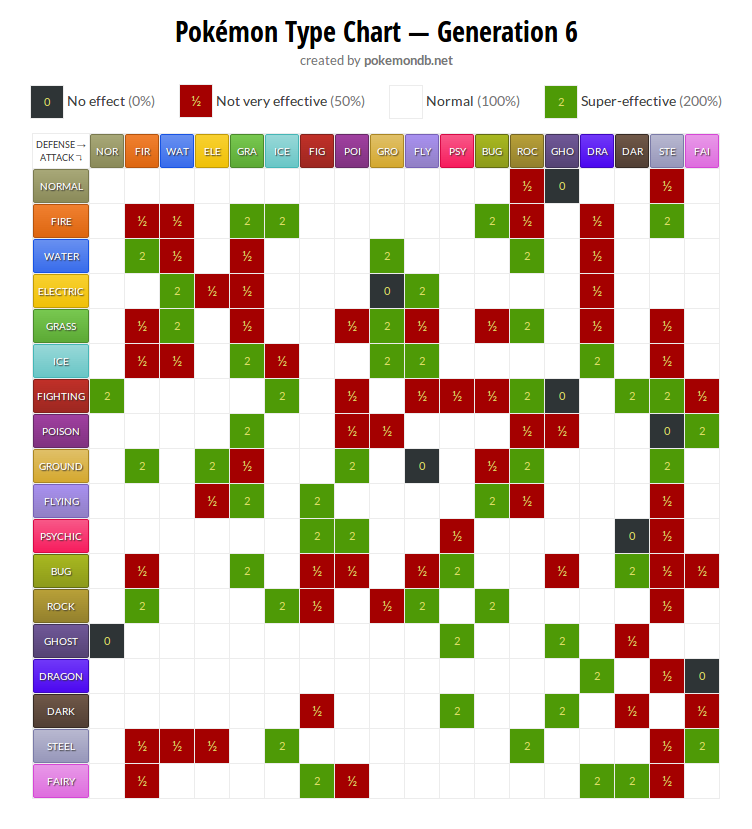
\includegraphics[width=0.85\textwidth]{img/typechart.png}
\caption{\label{fig:schema}Charte graphique des types, de leur forces et faiblesses, pokemondb.net/type}
\end{figure}

\subsubsection{Les statistiques du Pokémon}

Le Pokémon contient aussi des statistiques qui vont influencer sur ses dégâts infligés et subis et/ou sa viabilité en combat ou hors-combat. Dans cette section, nous allons décrire toutes les variables qui compose le Pokémon.

\begin{enumerate}
    \item Les points de vie
    
Un Pokémon a un nombre de point de vie maximale, qu'il ne peut pas dépasser. Si ses points de vie tombent à zéro, le Pokémon feint et n'est plus disponible pour se battre.

    \item L'Attaque
    
L'Attaque affecte les capacités physique du Pokémon. Elle intervient lors de l'affectation des points de dégâts infligés.

    \item L'Attaque Spécial
    
L'Attaque Spéciale affecte les capacités spéciale du Pokémon. Elle intervient lors de l'affectation des points de dégâts infligés.

    \item La Défense
    
La Défense affecte les capacités physique du Pokémon. Elle intervient lors de l'affectation des points de dégâts subis.

    \item La Défense Spéciale
    
La Défense Spéciale affecte les capacités spéciale du Pokémon. Elle intervient lors de l'affectation des points de dégâts subis.

    \item La Vitesse
    
La Vitesse détermine l'ordre d'action des Pokémons en combat. Sauf sous certaines exceptions, un Pokémon A dont la vitesse est supérieure à un Pokémon B attaquera en premier dans le tour.

    \item Les statistiques de base
    
Chaque Pokémon a des statistiques de base qui lui sont propres. Les statistiques notées ci-dessus peuvent fluctuer selon certains facteurs dont les statistiques de base du Pokémon concerné. Les statistiques de base ne changeront pas durant la progression du Pokémon.

    \item Les Points Individuelles - IV
    
Les points individuelles, ou IV, sont déterminées à la naissance du Pokémon ou lors de sa rencontre dans la nature. Les IV sont générées de manière dans chaque statistiques du Pokémon (Points de vie, Attaque, Attaque Spéciale, Défense, Défense Spéciale et Vitesse) et ils ne peuvent pas changer. Le total maximale des IV d'un Pokémon ne peut pas dépasser 186, et ne peut pas dépasser 31 d'IV par statistiques.

    \item Les Points d'Efforts - EV
    
Chaque fois qu'un Pokémon A bat un Pokémon B, le Pokémon A va recevoir un EV dans une statistique précise qui dépend du Pokémon B. Tout les 4 EV dans une statistique, la statistique augmente d'un point. En total, un Pokémon peut obtenir 510 EV, et 255 EV maximum dans une seule statistique.

\end{enumerate}

\subsubsection{La nature du Pokémon}

La nature pour les Pokémon est apparu à la troisième génération. Une nature peut soit être neutre, et n'avoir aucun effet sur le Pokémon, ou alors peut affecter un bonus et un malus de statistiques au Pokémon affligé. Ce bonus et ce malus sont toujours de 10\% de deux statistiques différentes. L'attribution de la nature est aléatoire à la création du Pokémon. Il existe cependant des moyens pour influencer la nature d'un Pokémon au travers de mécaniques de jeu.

Il existe 25 natures différentes dont 5 qui sont neutres. Par raison de visibilité, je vais séparer les différents tableaux selon les bonus offerts par la nature.

Tableau des natures d'attaque :

\begin{tabular}{c c c c c c}
    \textbf{Nature} & \textbf{Attaque} & \textbf{Défense} & \textbf{Attaque Spéciale} & \textbf{Défense Spéciale} & \textbf{Vitesse}\\
    \hline
    Brave & +10\% & - & - & - & -10\%\\
    Mauvais & +10\% & - & - & -10\% & -\\
    Rigide & +10\% & - & -10\% & - & -\\
    Solo & +10\% & -10\% & - & - & -\\
\end{tabular}

Tableau des natures de défense :

\begin{tabular}{c c c c c c}
    \textbf{Nature} & \textbf{Attaque} & \textbf{Défense} & \textbf{Attaque Spéciale} & \textbf{Défense Spéciale} & \textbf{Vitesse}\\
    \hline
    Assuré & -10\% & +10\% & - & - & -\\
    Lâche & - & +10\% & - & -10\% & -\\
    Malin & - & +10\% & -10\% & - & -\\
    Relax & - & +10\% & - & - & -10\% \\
\end{tabular}

Tableau des natures d'attaque spéciale :

\begin{tabular}{c c c c c c}
    \textbf{Nature} & \textbf{Attaque} & \textbf{Défense} & \textbf{Attaque Spéciale} & \textbf{Défense Spéciale} & \textbf{Vitesse}\\
    \hline
    Discret & - & - & +10\% & - & -10\%\\
    Doux & - & -10\% & +10\% & - & -\\
    Foufou & - & - & +10\% & -10\% & -\\
    Modeste & -10\% & - & +10\% & - & -\\
\end{tabular}

Tableau des natures de défense spéciale :

\begin{tabular}{c c c c c c}
    \textbf{Nature} & \textbf{Attaque} & \textbf{Défense} & \textbf{Attaque Spéciale} & \textbf{Défense Spéciale} & \textbf{Vitesse}\\
    \hline
    Calme & -10\% & - & - & +10\% & -\\
    Gentil & - & -10\% & - & +10\% & -\\
    Malpoli & - & - & - & +10\% & -10\%\\
    Prudent & - & - & -10\% & +10\% & -\\
\end{tabular}

Tableau des natures de vitesse :

\begin{tabular}{c c c c c c}
    \textbf{Nature} & \textbf{Attaque} & \textbf{Défense} & \textbf{Attaque Spéciale} & \textbf{Défense Spéciale} & \textbf{Vitesse}\\
    \hline
    Jovial & - & - & -10\% & - & +10\%\\
    Naïf & - & - & - & -10\% & +10\%\\
    Pressé & - & -10\% & - & - & +10\%\\
    Timide & -10\% & - & - & - & +10\%\\
\end{tabular}

Tableau des natures neutre :

\begin{tabular}{c c c c c c}
    \textbf{Nature} & \textbf{Attaque} & \textbf{Défense} & \textbf{Attaque Spéciale} & \textbf{Défense Spéciale} & \textbf{Vitesse}\\
    \hline
    Bizarre & - & - & - & - & -\\
    Docile & - & - & - & - & -\\
    Hardi & - & - & - & - & -\\
    Pudique & - & - & - & - & -\\
    Sérieux & - & - & - & - & -\\
\end{tabular}

\subsubsection{Le talent du Pokémon}

Le talent, ou capacité spéciale, d'un Pokémon est un effet qui agit en combat et depuis la version Èmeraude, peut aussi agir en dehors des combats. Le talent est une mécanique de jeu qui est apparu avec la troisième génération des jeux Pokémon. Depuis la cinquième génération, les talents cachés ont vu le jour, il s'agit de talents que les Pokémon affectés ne possèdent pas naturellement. Depuis la septième génération, il est possible pour un Pokémon de posséder plusieurs talents. À l'heure actuelle, il existe prés de 200 talents.

Ces talents peuvent s'activer à différentes occasions :

\begin{itemize}
    \item lorsque le Pokémon arrive en combat
    \item entre chaque tour
    \item en permanence
    \item lors de son attaque
    \item lors d'une attaque adverse
    \item selon les points de vie restants
    \item selon le climat
    \item après un combat
\end{itemize}

À cela s'ajoute les différentes catégories de talents qui classifie sur quoi elles interviennent ou interagissent avec :

\begin{itemize}
    \item Talents du climats
    \item Talents des champs
    \item Immunités et conversions
    \item Talents qui diminuent les dégâts
    \item Talents qui augmentent les dégâts de certains attaques
    \item Talents qui bloquent les baisses de statistiques
    \item Talents qui bloquent les changements de statut
    \item Talents qui s'activent lors d'un changement de statut
    \item Talent qui a un effet sur le terrain
    \item Talent qui modifie une statistique
    \item Talents qui modifient le types des attaques
    \item Talents qui s'activent lors d'une attaque directe
    \item Talents de soin
    \item Talents handicapant
    \item Talents influant sur la vitesse des attaques
    \item Talents de transformation
    \item Talents signatures, qui sont unique à une espèce de Pokémon
\end{itemize}

\subsubsection{Les capacités du Pokémon}

Les capacités du Pokémon vont être ce qui va lui permettre de s'opposer à son adversaire en combat. Chaque Pokémon peut avoir jusqu'à quatre capacité différentes.

Une capacité est composé de différents critères et statistique qui vont l'impacter :

\begin{itemize}

    \item Le type
    
    Le type des attaques suit la même philosophie que le type des Pokémon. Voir {\ref{type_pokemon}}.
    
    \item Les points de pouvoirs
    
    Les points de pouvoir déterminent combien de fois l'attaque peut être lancé avant que la capacité ne devienne inutilisable en combat. Ils peuvent bien évidemment être régénéré par le biais d'objet ou simplement par le soin complet d'un Pokémon.
    
    \item Les dégâts
    
    Une capacité offensive peut infliger des dégâts. Ses dégâts sont en général comptés dans une fourchette allant d'un minimum de dégâts X à un maximum Y. Entre cette fourchette est déterminé un nombre aléatoire qui va déterminer les dégâts que cette attaque va infliger. 
    
    \item La précision
    
    Toutes capacités confondues ont une chance de rater leur cible due à leur précision. La précision d'une capacité détermine le pourcentage de chance d'une capacité à toucher sa cible.
    
    \item L'effet
    
    La capacité peut appliquer un effet sur sa cible. Cet effet influe sur ses statistiques.
    
    \item La catégorie
    
    La catégorie d'une attaque spécifie quel statistique des Pokémon attaquant et défendeur vont utiliser.
    
    \begin{itemize}
    
        \item Physique
        
        Dans le cas d'une capacité physique, l'attaquant utilisera l'Attaque et le défendeur utilisera la Défense.
        
        \item Spéciale
        
        Dans le cas d'une capacité spéciale, l'attaquant utilisera l'Attaque Spéciale et le défendeur utilisera la Défense Spéciale.
        
        \item de statut
        
        Les capacités de statut en revanche n'utilisent pas de statistique pour avoir un effet sur le défendeur.
        
    \end{itemize}
    
    \item Capacité Z
    
    Les capacités Z sont des capacités souvent améliorés d'une capacité existante. Il peut toutes fois s'agir aussi d'une capacité unique à un Pokémon, ce qui lui nécessitera de porter un objet particulier pour accomplir l'activation de cette capacité.
    
\end{itemize}
    
\subsubsection{Le statut du Pokémon}

Un Pokémon peut être affliger par un statut qui va impacter sur sa performance. On considère qu'il y a deux grandes familles de statut :

\begin{enumerate}

    \item Principales
    
    La famille principale de statut corresponds aux statuts qui vont affecter le Pokémon en combat ainsi qu'hors-combat. Un statut étant principale sera affiché sur le Pokémon. Un Pokémon ne peut pas être affecté par plus d'un statut principale à la fois. Après un certain nombre de tours, le statut peut disparaître.
    
    \begin{itemize}
    
        \item Brûlure
        
        Chaque tour, un Pokémon affligé par Brûlure subira des dégâts de feu.
    
        \item Gel
        
        Tant qu'un Pokémon est gelé, il ne peut rien faire. À partir d'un certain nombre de tour, ce statut peut disparaître.
    
        \item Paralysie
        
        Si un Pokémon est paralysé, à chaque action qu'il est sur le point d'effectuer, il y a des chances qu'il ne puisse pas la réaliser.
    
        \item Empoisonnement
        
        Chaque tour, un Pokémon affligé par Empoisonnement subit des dégâts de poison.
        
        En dehors des combats, un Pokémon empoisonné prendra des dégâts de poison après un certain nombre de pas dans le monde.
    
        \item Sommeil
        
        Tant qu'un Pokémon est endormi, il ne peut rien faire. À partir d'un certain nombre de tour, ce statut peut disparaître.
        
    \end{itemize}

    \item Secondaires
    
    Un statut secondaire n'affectera pas le Pokémon hors-combat et est retiré lorsque le Pokémon n'est plus en combat (donc dans le cas où le Pokémon est échangé pour un autre durant un combat ou lorsque le combat est terminé). Un Pokémon peut être affligé par autant de statut secondaire qu'il n'y en a, et peut aussi souffrir d'un statut principale en même temps.
    
    \begin{itemize}
    
        \item Attraction
        
        Un Pokémon A peut être attiré par un Pokémon B, sous condition que le Pokémon A et B sont de sexes différents. Un Pokémon affligé par Attraction refusera d'attaquer le Pokémon qui lui aura donné le statut en premier lieu. À partir d'un certain nombre de tour, ce statut peut disparaître.
    
        \item Confusion
        
        Quand un Pokémon est confus, il y a des chances que lorsqu'il tentera une action, il s'inflige des dégâts à lui-même sans réaliser l'action qu'il allait entreprendre. À partir d'un certain nombre de tour, ce statut peut disparaître.
    
        \item Malédiction
        
        Un Pokémon A de type Spectre peut sacrifier la moitié de ses points de vie afin de maudire un Pokémon B. Le Pokémon B va, suite à la réussite du Pokémon A, perdre le quart de ses points de vie chaque tour.
    
        \item Peur
        
        Un Pokémon affligé par peur ne peut pas attaquer durant son tour. Peur ne dure qu'un seul tour.
    
        \item Clairvoyance, Flair, Oeil Miracle
        
        Un Pokémon ayant Clairvoyance, Flair ou Oeil Miracle ne verra pas la précision de ses attaques affecté pas les changements de l'Esquive d'un Pokémon adverse. 
        
        De plus, si le Pokémon a utilisé Clairvoyance ou Flair ses attaques de types Normal et Combat affecteront les Pokémon de type Spectre, et il a utilisé Oeil Miracle, ses attaques Psy affectent les Pokémon de type Ténèbres.
    
        \item Piège
    
        \item Désobéissance
    
        \item Vampigraine
        
    \end{itemize}
    
\end{enumerate}
        
\subsubsection{L'esquive du Pokémon}

Esquive

\subsubsection{La forme du Pokémon}

Forme
    Permanente
    Combat
    En/Hors Combat
    
\subsubsection{Autres}

Poids

Bonheur
    

\subsection{Extérieur au Pokémon}

\subsubsection{Le climat}

Climat
    Ensoleile
        Soleil intense
    Pluie
        Pluie batante
    Grele
    Tempete de sable
    Brouillard
    Souffle delta

\subsubsection{Le champ actif}

Champ

\subsubsection{Les objets}

Objets tenus
Objets dans le sac
    Hors-Combat
    En combat

\section{Format VGC}

Le tournoi
Définisse le format : 2vs2, etc
Le jeu utilisé
    -> Limite les pokémons utilisable
    -> Limite les capacités utilisable
    -> Limite les objets utilisable


\section{Pour notre goal}